\section{Basic Antenna Parameters}
\label{sec:basicantennaparams}
This section will give a summery of the fundamental theories and parameters that are used to describe antennas. This should give a basic understanding of antennas. The parameters described in this section are used throughout the report. 

\subsection{Antenna Definition}
\label{subsec:antenna-def}
The IEEE defines an antenna as: ``a means for radiating or receiving radio waves''. In other words, the purpose of an antenna is to make the transition from a signal in a transmission line to electromagnetic fields in the air. An antenna will radiates an electric field (E-field) in a given direction, which then induces a magnetic field (H-field) orthogonal to the E-field, this relation is described by Maxwell's Equations which is covered in Section~\ref{sec:fdtd} \cite{balanis2012antenna}.

\subsection{Isotropic Radiator}
\label{subsec:isotropic-ant}
An isotropic antenna, can be represented as a point source. The isotropic antenna radiates its power uniformly in a sphere. The power density $S_{\text{iso}}$ can be expressed as the source power $P_s$ over the surface area of a sphere which is given by $4\pi r^2$ \cite{balanis2012antenna}:
\begin{align}
    S_{\text{iso}} = \frac{P_s}{4\pi r^2}
\end{align}
Clearly, it is not possible to construct such an antenna. However, this is used as a reference for quantifying other properties of the antenna. These properties could be the gain or directivity (See Section \ref{subsec:dir_gain}), and the unit would then be in \si{dBi} rather than \si{dB}.

\subsection{Radiation Pattern}
\label{subsec:radiation-p}
The radiation pattern describes how the antenna emits or receives radiated power. This is commonly visualized by a 3D plot or 2D cuts of the 3D plot in specific coordinates. The unit of power used is often gain or directivity (See Section~\ref{subsec:dir_gain}) and this is often compared to the isotropic antenna \cite{balanis2012antenna}.

\subsection{Field Regions}
The waves transmitted from the antenna are usually grouped into three regions of radiation, based on how the waves propagate and the field structure \cite{balanis2012antenna}. Obviously, there is no abrupt change, but rather a continuous change.
\begin{itemize}
\item The Reactive near-field 
\item The Radiating near-field (Fresnel)
\item The Far-field
\end{itemize}

The reactive near-field is defined as the portion of the near-field region immediately surrounding the antenna wherein the reactive field predominates \cite{balanis2012antenna}. The outer boundary for this region is given by \cite{balanis2012antenna}:
\begin{align}
  R < 0.62 \sqrt{D^3/\lambda}
\end{align}

The radiating near-field is defined as the region between the reactive near-field and the far-field, this field might not exist in the case that the overall antenna dimension is very small compared to the wavelength. The outer boundary for this is defined as \cite{balanis2012antenna}:
\begin{align}
  R \geq 2D^2/\lambda
\end{align}

The far-field region is defined as the region of the field where the angular field distribution is independent of the distance, that is the radiation pattern does not change shape with distance. The far-field is also dominated by fields where the E- and H-fields are orthogonal and propagates as plane waves. The inner boundary is given as \cite{balanis2012antenna}:
\begin{align}
  R = 2D^2/\lambda
\end{align}

These different regions are illustrated on Figure~\ref{fig:field-regions}. 

\begin{figure}[htbp]
  \centering
  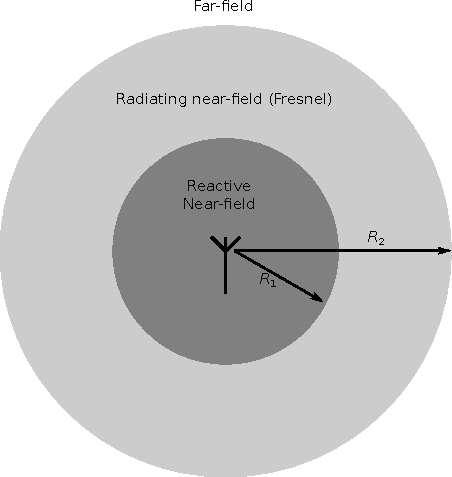
\includegraphics[scale=1]{img/analysis/radiationfields}
  \caption{Visualization of different fields \cite{balanis2012antenna}.}
  \label{fig:field-regions}
\end{figure}

\subsection{Directivity and Gain}
\label{subsec:dir_gain}
Directivity is defined as the ratio of the power radiated at a  point with a certain angle and distance from the antenna compared to what would be radiated from a reference isotropic antenna. Mathematically, it can be written as \cite{balanis2012antenna}: 
\begin{align}
  D = \frac{U}{U_0} = \frac{4 \pi U}{P_{rad}} 
\end{align}
where
\begin{where}
  \item[$D$] directivity
  \item[$U$] radiation intensity
  \item[$U_0$] radiation intensity of an isotropic source
  \item[$P_{rad}$] total radiated power 
\end{where}
It should be noted, that for this equation to be valid, the waves must propagate as plane waves, thus being in the far-field region.

Gain is a measure closely related to directivity, it takes the antenna efficiency of the antenna into account as well as the direction. The gain is defined as the ratio of the intensity in a given direction to the radiant intensity that would be obtained if it was radiated isotropically. In mathematical form it can be expressed as \cite{balanis2012antenna}:
\begin{align}
  G = 4 \pi \frac{\text{radiation intensity}}{\text{total accepted input power}} = 4 \pi \frac{U(\theta,\phi)}{P_{in}}
\end{align}
In many cases the relative gain is used, which is defined as the ratio of the power gain in a given direction to the power gain of a reference antenna in its referenced direction. The reference antenna could be a dipole, horn etc. 

The gain can also be calculated using the directivity, since they are only related by the efficiency. This is given as \cite{balanis2012antenna}:
\begin{align}
  G(\theta,\phi) = e_{cd}D(\theta, \phi) 
\end{align}

\subsection{Impedance, Return Loss, and VSWR}
The impedance and matching is an important part of the antenna design to ensure maximum power transfer. The input impedance of an antenna is defined as $Z_{\text{in}}$. From the classical circuit theory it is known that the maximum power transfer occurs when the in- and output impedance is matched (see Section~\ref{sec:tuners}). If there is a mismatch, some of the power will be reflected back into the source, and thus not transmitted from the antenna. The reflection coefficient $\Gamma$ is defined as \cite{pozar2011microwave}:
\begin{align}
    \Gamma = \frac{Z_{\text{in}}-Z_0}{Z_{\text{in}}+Z_0} 
\end{align}
where
\begin{where}
\item[$Z_0$] denotes the characteristic impedance, which is typically \SI{50}{\ohm}.
\end{where}
The reflection coefficient is furthermore often expressed in \si{dB}. 

Another closely related figure is the Voltage Standing Wave Ratio (VSWR), and is defined as \cite{pozar2011microwave}: 
\begin{align}
  \text{VSWR} = \frac{1+|\Gamma|}{1-|\Gamma|}
\end{align}

\subsection{Bandwidth}
The bandwidth of an antenna defines the usable spectrum of the antenna. The needed bandwidth is dependent on the modulation schemes used, which makes the bandwidth an important part of the antenna design. The bandwidth is defined with respect to a given reflection coefficient or VSWR.

\subsection{Polarization}
The polarization in a certain direction is simply defined as the polarization of the transmitted wave by the antenna. It describes the time-varying direction at relative magnitude of the E-field vector analogously to the polarization of light. Similar to light, the polarization can be classified into groups such as linear, circular, or elliptical polarization. If two antennas are of different polarization, this will introduce a polarization mismatch loss to the system \cite{balanis2012antenna}.

\subsection{Antenna Efficiency}
There are a lot of different measures for antenna efficiency depending on which losses that are taken into account. The total efficiency takes the losses from the input terminal and within the antenna structure \cite{balanis2012antenna}. This can in general be expressed as \cite{balanis2012antenna}
\begin{align}
\label{eq:ant-eff}
  e_0 = e_r e_c e_d 
\end{align}
where
\begin{where}
\item[$e_0$] total efficiency.
\item[$e_r$] mismatch loss.
\item[$e_c$] conduction efficiency.
\item[$e_d$] dielectric loss.
\end{where}
The conduction and dielectric losses are hard to compute, and by measurements they cannot be separated \cite{balanis2012antenna}.

\subsubsection{Radiation Efficiency}
The radiation efficiency is defined as the conduction-dielectric efficiency $e_r = e_{cd}$ which is defined as the ratio of the power delivered to the radiation resistance, $R_r$, to the power delivered to $R_r$ and $R_L$ \cite{balanis2012antenna}. This can be written as \cite{balanis2012antenna}:
\begin{align}
  e_r = \frac{P_{\text{radiated}}}{P_{\text{input}}} = \frac{R_r}{R_L+Rr}
\end{align}

\subsection{Antenna Q Factor}
The antenna Q factor (Quality factor) is often used to get an estimation of the bandwidth of a given antenna. The definition of the Q factor of an antenna is defined in Equation~\ref{eq:antenna-q-factor} below \cite{fundamentalMcLean}: 
\begin{align}
  \label{eq:antenna-q-factor}
      Q =
    \begin{dcases}
       \frac{2 \omega W_e}{P_{\text{rad}}} & W_e > W_m  \\
       \frac{2 \omega W_e}{P_{\text{rad}}} & W_m > W_e 
    \end{dcases}
\end{align}
where 
\begin{where}
\item[$W_e$] the time-average non-propagating stored electric energy.
\item[$W_m$] the same as the above just with magnetic energy.
\item[$\omega$] the radian frequency and $P_{\text{rad}}$ denotes the radiated power.
\end{where}

\subsection{Electrically Small Antennas}
The concept and definition of electrically small antennas was introduced by Wheeler in 1947 \cite{wheeler1947}, and is given by:
\begin{align}
\label{eq:esa-def}
  ka \ll 1
\end{align}
where 
\begin{where}
\item[$k$] $\frac{2\pi}{\lambda}$ is the wave number. 
\item[$a$] the radius of a sphere enclosing the maximum dimension of the antenna. 
\end{where}
The parameter $a$ is illustrated in Figure~\ref{fig:ant-esa-def}. Inserting the definition of $k$ yields that
\begin{align}
  \frac{2\pi a}{\lambda} \ll 1
\end{align}
in order for an antenna to be defined as electrically small. It should also be noted that, if the antenna is used with a small ground plane, which often is the case, then the ground plane it self becomes a dominant part of the antenna structure. In this case, the entire ground plane must be included in the sphere and thus in the definition of $a$.

\begin{figure}[htbp]
  \centering
  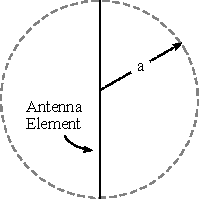
\includegraphics[scale=1]{img/analysis/ESA}
  \caption{Illustration of ESA definition \cite{}}
  \label{fig:ant-esa-def}
\end{figure}


\subsubsection{Fundamental limits of Q}
L.J.\ Chu quantified the relationship between the minimum Q of an electrically small antenna and the physical size relative to the wavelength \cite{chu1948}. This relationship was later corrected by McLean \cite{mclean1996} to be: 
\begin{align}
  Q_L = \frac{1}{k^3a^3}+ \frac{1}{ka}
\end{align}
For a linear antenna in free space and for a circular polarized antenna \cite{mclean1996}:
\begin{align}
  Q_{cp} = \frac{1}{2}  \left[ \frac{1}{k^3a^3} + \frac{2}{ka} \right] 
\end{align}

\subsection{Friis Transmission Equation}
The Friis transmission equation relates the power received with the power transmitted. In the most simple form the Friis transmission equation is based on the Free-space path loss (FSPL), the gains of the antennas and the transmit power. The free-space path loss (or ``path gain'' as this is a negative notation) is defined as \cite{balanis2012antenna}
\begin{align}
  \label{eq:fspl}
  \text{FSPL} = \left( \frac{\lambda}{4 \pi d} \right)^2 
\end{align}
where
\begin{where}
\item[$\lambda$] wavelength.
\item[$d$] distance from the transmitter.
\end{where}
This assumes that the energy spreads out in a sphere and that the only loss is from the distance. It is seen that the power decreases as the square of the range, which is plotted on Figure~\ref{fig:fspl-plot} for a \SI{2.6}{GHz} link.

\begin{figure}[htbp]
  \centering
  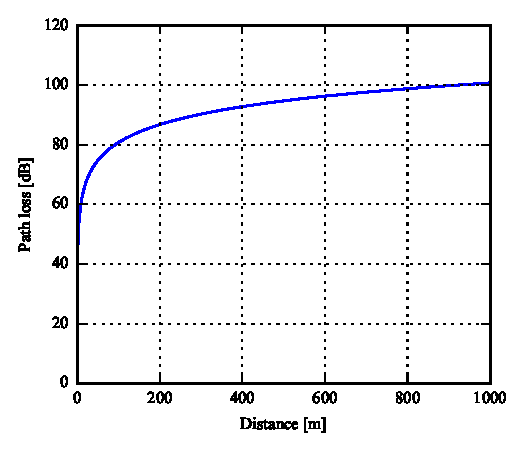
\includegraphics{img/analysis/distancePathloss}
  \caption{Free space path loss in dB for a \SI{2.6}{GHz} link.}
  \label{fig:fspl-plot}
\end{figure}

The Friis Transmission equation in its most basic form can be written as \cite{balanis2012antenna} 
\begin{align}
    \frac{P_r}{P_t} = \left( \frac{\lambda}{4 \pi d} \right)^2 G_{t} G_{r} 
\end{align}
where
\begin{where} 
\item[$P_r$] power received.
\item[$P_t$] power transmitted.
\item[$G$] transmitter and receiver gains.
\end{where}
In this case it is assumed that there is no impedance or polarization mismatch. It is also assumed that the two antennas are aligned perfectly. Another large assumption is that the path loss is described by FSPL, which in reality is a very rare case. The next section will describe a few different propagation models.

\section{Basic Propagation Models}
\label{sec:propmodels}
This section will describe some simple propagation models and terms, that can be used to establish a rough estimate of the losses from propagation, which can be used in link budgets. The simplest propagation model is the Free space path loss, which is given in Equation~\ref{eq:fspl}.

The free-space path loss is however not very realistic, since it does not take trees, buildings etc. into account \cite{balanis2012antenna}. There are however a myriad of empirical models, which are based on actual measurements. The drawback is however that these empirical models tend not to be general and a given model might not be suited for two different cities. This results in that empirical models often are grouped into three main branches, foliage, terrain and city models \cite{goldsmith2005wireless}. For foliage areas models such as the Weissbergers model and the ITU Vegetation model can be used \cite{goldsmith2005wireless}. For terrain areas, models such as the Egli or Longley-Rice model are used \cite{goldsmith2005wireless}. To model the path loss in cities, the Young, Okumura, Hata or the COST 231 models can be used \cite{goldsmith2005wireless}. It should be noted that some of these models are not usable in upper LTE frequency range, and thus care should be taken when applying these models. 


\subsection{Multipath}
The multipath effect exists when a wave and/or multiple waves are scattered, such that the receiver experiences multiple copies of the same wave coming from different directions. In areas where there is no ground or other obstacles (free space) the multipath effect does not exist. The simplest multipath case is the two-ray case, where the surface of the earth is included, in this case there will be a single reflection from the earth and thus multiple paths from the transmitter to receiver \cite{parsons2000mobile}. This scenario is illustrated in Figure~\ref{fig:mul_tworay}.
 
\begin{figure}[htbp]
    \centering
    \begin{subfigure}[b]{0.6\textwidth} 
        \centering
        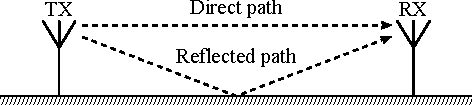
\includegraphics{img/analysis/tworay}
        \caption{Two ray path model.}
        \label{fig:mul_tworay}
    \end{subfigure}
    \\
    \begin{subfigure}[b]{0.7\textwidth} 
        \centering
        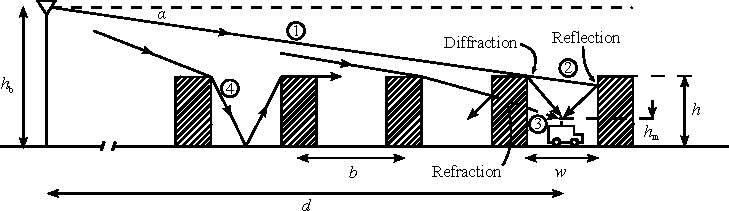
\includegraphics{img/analysis/parsons_multipath}
        \caption{Reflection and diffraction causing the multi-path effect \cite{parsons2000mobile}. The signal received by the car consists of diffracted, reflected, and refracted waves but no direct line-of-sight component.}
        \label{fig:mul_reflec_diffrac}
    \end{subfigure}
    \caption{Two ray model and different multipath effects.}
\end{figure}

The multipath effect will be greatest in urban environments, where several buildings and other obstacles are present. If the surface is rough, scattering will also take place. This is the phenomenon where a single incoming wave scatters into multiple reflections. In addition to this there is also diffraction where a wave front is ``bend'' at the edges of buildings which is illustrated in Figure~\ref{fig:mul_reflec_diffrac}. Multipath results in a negative effect on the throughput. However, with MIMO, the multipath effects are now exploited positively to increase throughput and channel stabilization \cite{parsons2000mobile}.

\subsection{Fading}
The signal strength in a wireless channel is constantly fluctuating. These variations are represented by fading. The variations can be caused by scattering, reflections, blockage etc. Based on the type of variation the fading is grouped in \emph{small scale fading} and \emph{large scale fading}. Large scale fading is typically caused by large objects, such as hills and buildings, where small scale fading occurs over small travel distances due to constructive or destructive adding of the multipath waves \cite{parsons2000mobile}.

By superimposing the path loss with small scale fading and large scale fading, the combined model is obtained which represents the total propagation and path loss model. This is illustrated in Figure \ref{fig:mul_combined}. 

\begin{figure}[htbp]
    \centering
    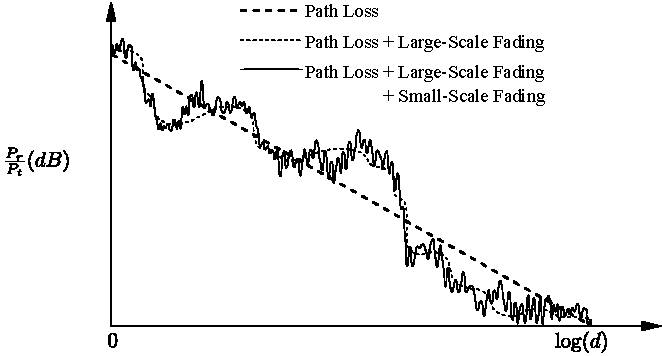
\includegraphics{img/analysis/goldsmith_combined}
    \caption{Combined path loss model with large- and small-scale fading \cite{goldsmith2005wireless}.}
    \label{fig:mul_combined}
\end{figure}

\subsection{Empirical Models}
This section will describe some of the city-models, that are often used in estimating the pathloss. 

\subsubsection{Hata Model}
The Hata model is a mathematical model derived from the graphically Okumura model, which is based on measurements from Tokyo in 1960 in the frequency range \SIrange{200}{1920}{MHz}. The model is divided into three groups: Urban, suburban, and open areas which are defined in dB in Equation~\ref{eqn:hataModelUrban}, Equation~\ref{eqn:hataModelSubUrban}, and Equation~\ref{eqn:hataModelOpen} respectively \cite{Seybold2005introduction}.
\begin{align} 
    \label{eqn:hataModelUrban}
    L_{50} = L_{50}(\text{urban}) = 69.55+26.12 \log(f_c) - 13.28 \log(h_t) -a(h_r) + [44.9-6.55 \log(h_t)] \log(d)
\end{align} 
where
\begin{where}
\item [$f_{c}$] Center frequency in \si{MHz} and in the range: $150 < f_c < 1500$
\item [$h_t$] Height in meters, which must satisfy $30 < h_t < 200$
\item [$d$] Distance in km which must satisfy $1 < d < 20$
\item [$a(h_r)$] The mobile antenna height correction factor. Defined in Equation~\ref{eqn:hataModelahrSmall} \cite{Seybold2005introduction} for small and medium sized cities. Defined in Equation~\ref{eqn:hataModelahrLarge} \cite{Seybold2005introduction} for a large city. 
\end{where}
\begin{align} 
\label{eqn:hataModelahrSmall}
a(h_r) &= [1.1 \log(f_c)-0.7]h_r - [1.56 \log(f_c)-0.8]\quad\text{if } \SI{1}{m} \leq h_r \leq \SI{10}{m} \\
\label{eqn:hataModelahrLarge}
a(h_r) &= 
  \begin{cases}
    8.29[\log(1.54 h_r))^2 -1.1 & \text{ if } f_c \leq \SI{200}{MHz}, \\
    3.2[\log(11.75 h_r))^2 -4.97 & \text{ if } f_c \leq \SI{400}{MHz} 
  \end{cases}\\
\label{eqn:hataModelSubUrban}
L_{50} &= L_{50}(\text{urban})-4.78[\log(f_c)]^2 + 18.33 \log(f_c) - 40.94 \\
\label{eqn:hataModelOpen}
L_{50} &= L_{50}(\text{urban})-2 \left[\log\left( \frac{f_c}{28} \right) \right]^2 -5.4 
\end{align} 
This extension to the Okumura model is often used in practical applications since it is easier to apply than the Okumura model. However, it only handles frequencies up to \SI{1500}{MHz}, which lead to the COST 231 model being developed. 

\subsubsection{COST 231 Model}
%COST 231 Model
The COST 231 model is an extension of the Hata model. It includes the PCS bands \SIrange{1800}{1900}{MHz} which makes it an ideal model for many wireless personal communication systems (GSM etc.). The path loss is given by Equation~\ref{eqn:COSTModel} in dB \cite{Seybold2005introduction} and the model is valid in the frequency range of  \SIrange{1500}{2000}{MHz}, link distance of up to \SI{20}{km}, a transmitter antenna height of \SIrange{30}{200}{m}, and a receiver height of \SIrange{1}{10}{m} \cite{Seybold2005introduction}. It should also be stated that the model is restricted to applications where the base station antenna is above adjacent roof tops \cite{itu2002report}.
\begin{align} 
    \label{eqn:COSTModel}
    L_{50} = 46.3+33.9 \log(f_c)-13.82 \log(h_t)-a(ht)+[44.9-6.55 \log(h_t)] \log(d) + C 
\end{align} 
where 
\begin{where}
\item [$f_c$] The frequency in \si{MHz}.
\item [$h_t$] Transmitter height in \si{m}. 
\item [$h_r$] Receiver height in \si{m}.
\item [$a(h_r)$] The mobile antenna height correction factor from Equation~\ref{eqn:hataModelahrSmall} and Equation~\ref{eqn:hataModelahrLarge}.
\item [$d$] Distance of propagation.
\item [$C$] \SI{0}{dB} for suburban and medium cities with medium tree density, 3 dB for metropolitan centers. 
\end{where}

\subsubsection{Extended COST}
%Extended COST 
An extension to the COST 231 model is described in a ITU (International Telecommunication Union) report \cite{itu2002report} and this model extends the COST 231 such that it is accurate up to \SI{3}{GHz}. The path loss model for an urban environment in the range of \SIrange{2000}{3000}{MHz} is given by \cite{itu2002report}
\begin{equation} 
\label{eqn:COSTModelExtended}
\begin{aligned}
    L &= 46.3 + 33.9 \log(2000) + 10 \log\left(\frac{f_c}{2000}\right) \\
        &- 13.82 \log(\text{max}\{30,h_t\}) + [44.9 -6.55 \log(\text{max}\{30,h_t\})] (\log(d))^{\alpha} - a(h_r) - b(h_t)
%L = 46.3 + 33.9\log(2000) + 10\log(\frac{f_c}{2000}) − 13.82\log(max{30,H_t}) +[44.9 − 6.55\log(max{30,H_t})](\log(d))\alpha −a(H_r)−b(H_t)
\end{aligned}
\end{equation} 
where 
\begin{where}
\item [$f_c$] The frequency in \si{MHz}.
\item [$h_t$] Transmitter height in \si{m}. 
\item [$h_r$] Receiver height in \si{m}.
\item [$a(h_r)$] The mobile antenna height correction factor given in Equation~\ref{eqn:COSTModelExtendedhr}
\item [$b(h_t)$] Transmitter height correction factor given in Equation~\ref{eqn:COSTModelExtendedht}
\item [$\alpha$] Given in Equation~\ref{eqn:aplhacostextended}.
\end{where}
\begin{align} 
\label{eqn:COSTModelExtendedhr}
a(h_r)&=(1.1\log(f)-0.7) \min\{10,h_r\}-(1.56\log(f)-0.8)+\max\left\{0,20\log\left(\frac{h_r}{10}\right)\right\}\\
\label{eqn:COSTModelExtendedht}
b(h_t)&= \min\left\{0,20\log\left(\frac{h_t}{30}\right)\right\}\\
\label{eqn:aplhacostextended}
\alpha &= 
  \begin{cases}
      1 & \text{ if } (d \leq \SI{20}{km}) \\
    1+(0.14+1.87e^{-4} f + 1.07e^{-3} h_t & \text{ if } (\SI{20}{km} < d \leq \SI{100}{km})
  \end{cases}
\end{align} 
